\documentclass[
    type = bachelor,
    degree = academic,
    twoside,
    fontset = win,
    decl-page
]
{njuthesis}

% njuthesis 参数设置文件 v1.4.0 2024-03-19

\njusetup[info]{
    title = {面向TLA\textsuperscript{+}规约的\\归纳不变式自动生成技术},
    title* = {Automatic Inductive Invariants Learning for TLA\textsuperscript{+} Specifications},
    author = {张继华},
    author* = {Jihua Zhang},
    keywords = {TLA\textsuperscript{+}, 分布式系统, 形式化验证, 强化学习, 归纳不变式},
    keywords* = {TLA\textsuperscript{+}, Distributed System, Formal Verification, Reinforcement Learning, Inductive Invariant},
    grade = {2020},
    student-id = {201250040},
    department = {软件学院},
    major = {软件工程},
    major* = {Software Engineering},
    supervisor = {魏恒峰,助理研究员},
    supervisor*= {Hengfeng Wei, Research Assistant},
    submit-date = {2024-05-20},
    % 提交日期
    supervisor-contact = {
        南京大学~
        江苏省南京市鼓楼区汉口路22号
    }
    % 导师联系方式
}

% bib 类用于参考文献设置
\njusetup[bib]{
    % style = numeric|author-year,
    % 参考文献样式
    % 默认为顺序编码制(numeric)
    % 可选著者-出版年制(author-year)
    %
    resource = {zhangjihua-thesis.bib},
    % 参考文献数据源
    % 需要带扩展名的完整文件名
    % 可使用逗号分隔多个文件
    % 此条等效于 \addbibresource 命令
    %
    % option = {
        % doi    = false,
        % isbn   = false,
        % url    = false,
        % eprint = false,
        % 关闭部分无用文献信息
        %
        % refsection = chapter,
        % 将参考文献表置于每章后
        %
        % gbnamefmt = lowercase
        % 使用仅首字母大写的姓名
    %   }
    % 额外的 biblatex 宏包选项
}

% image 类用于载入外置的图片
\njusetup[image]{
    % path = {{./figure/}{./image/}},
    % 图片搜索路径
    %
    nju-emblem = {nju-emblem},
    nju-name = {nju-name},
    % nju-emblem = {nju-emblem-purple},
    % nju-name = {nju-name-purple},
    % 替换为紫色版本
    % 这个选项只能填写一次
    % 切换时要注释掉上方的黑色版本
}

% abstract 类用于设置摘要样式
\njusetup[abstract]{
    toc-entry = true,
    % 摘要是否显示在目录条目中
    %
    % underline = false,
    % 研究生英文摘要页条目内容是否添加下划线
    %
    % title-style = strict|centered|natural
    % 研究生摘要标题样式,详见手册
}

% 目录自身是否显示在目录条目中
\njusetup{
    tableofcontents/toc-entry = false,
    % 关闭本项相当于同时关闭三个选项
    %
    % listoffigures/toc-entry   = false,
    % listoftables/toc-entry    = false
}

% 为目录中的章标题添加引导线
\njusetup[tableofcontents/dotline]{chapter}

% math 类用于设置数学符号样式,功能详见手册
\njusetup[math]{
    % style              = TeX|ISO|GB,
    % 整体风格,缺省值为国标(GB)
    % 相当于自动设置以下若干项
    %
    % integral           = upright|slanted,
    % integral-limits    = true|false,
    % less-than-or-equal = slanted|horizontal,
    % math-ellipsis      = centered|lower,
    % partial            = upright|italic,
    % real-part          = roman|fraktur,
    % vector             = boldfont|arrow,
    % uppercase-greek    = upright|italic
}

% theorem 类用于设置定理类环境样式,功能详见手册
\njusetup[theorem]{
    % define,
    % 默认创建内置的七种定理环境
    %
    % style         = remark,
    % header-font   = \sffamily \bfseries,
    % body-font     = \normalfont,
    % qed-symbol    = \ensuremath { \male },
    % counter       = section,
    % share-counter = true,
    % type          = {...}
    % 以上设置项在重新调用 theorem/define 后生效
}

% footnote 类用于设置脚注样式,功能详见手册
\njusetup[footnote]{
  % style = pifont|circled,
  % 使用圈码编号
  %
  % hang = false,
  % 不使用悬挂缩进
}

% 页眉页脚内容设置
\njusetup{
  % header/content = {
  %     {OR}{\thepage},{OL}{\rightmark},
  %     {EL}{\thepage},{ER}{\leftmark}
  %   },
  % 页眉设置,详见手册
  % 奇数页页眉:左侧章名,右侧页码
  % 偶数页页眉:左侧页码,右侧节名
  %
  % footer/content = {}
}

% 页眉页脚的字体样式
% \njusetformat{header}{\small\kaishu}
% \njusetformat{footer}{}

% 一些灵活调整
\njusetname{type}{本科毕业设计}                 % 我做的是毕业设计
% \njusetname{notation}{术语表}                   % 更改符号表名称
% \njusetlength{crulewd}{240pt}                   % 加长封面页下划线
% \njusetformat{tabular}{\zihao{-4}\bfseries}     % 修改表格环境的字号
% \EditInstance{nju}{u/cover/emblem-img}{align=l} % 左对齐的本科生封面校徽

\usepackage{listings} % 展示代码
\usepackage{algorithm,algorithmic} % 展示算法伪代码
\usepackage{subcaption} % 嵌套小幅图像,比 subfig 和 subfigure 更新更好
\usepackage{siunitx} % 标准单位符号
\usepackage{tabularx}
\usepackage{array}
\usepackage{booktabs}
\usepackage{appendix}
\usepackage{amsmath}

\lstset{
	frame=single,
        numbers=left,
	aboveskip=3mm,
	belowskip=3mm,
	showstringspaces=false,
	basicstyle=\footnotesize\ttfamily,
	columns=flexible,
	tabsize=2,
	keepspaces=true,
        breaklines=true,
        breakatwhitespace=true
}

\newcommand{\TLA}{TLA\textsuperscript{+}\ }

\begin{document}
% 封面
\maketitle

\begin{abstract}
    分布式协议以及分布式系统,在当今的计算机世界不可或缺。自动化地对分布式协议验证其正确性是一个重要且困难的挑战。
    为了验证分布式协议的正确性,我们可以尝试证明分布式协议的每一个状态都满足一个预先给定的不变式,即安全属性(safety property)。
    对于复杂系统,我们无法像验证简单系统,通过遍历所有状态的方式来验证安全属性。
    过去的研究中往往采用寻找一个蕴含着安全属性的不变式的方式来验证协议的正确性,这个不变式经过所有可能的状态转移后仍然能保持其自身的正确性。
    这个不变式被称为归纳不变式。
    自动化地生成分布式协议的归纳不变式是验证自动化分布式协议正确性的关键步骤。

    以往的研究主要基于的IVy进行实现,\TLA 语言领域的相关研究较少。本文将提供一种基于\TLA 的归纳不变式生成工具,实现对以\TLA 语言描述的分布式协议规约的归纳不变式的自动化生成。
    与此同时,通过引入了强化学习的方法,加速归纳不变式的推导。
    引入外部工具 \href{https://apalache.informal.systems/}{apalache} 作为验证引擎,实现了对归纳不变式的验证。
    在进入强化学习模块之前,我们基于 tla2tools 对 \TLA 源文件进行静态分析,提取出语义信息,以便强化学习框架理解 \TLA 文件的语义。
    通过实验,本文提出的方法的有效性和可行性可以得到验证。
\end{abstract}
  
\begin{abstract*}
    Distributed Protocols and distributed systems are indispensable in today's computer world. Automatically verifying the correctness of distributed protocols is an important and challenging task.
    To verify the correctness of distributed protocols, we can try to prove that every state of the distributed protocol satisfies a pre-defined invariant, a safety property.
    For complex systems, we cannot verify safety properties by traversing all states as we do for simple systems.
    Researchers often use the method of finding an invariant that implies the safety property, which remains correct after all possible state transitions. This invariant is called an inductive invariant.
    Automatically generating inductive invariants for distributed protocols is a key step in verifying the correctness of automated distributed protocols.

    Previous research is mainly based on IVy for implementation, few on \TLA. 
    This thesis will provide an inductive invariant generation tool based on \TLA, which realizes the automatic generation of inductive invariants for distributed protocol specifications described in \TLA language.
    Meanwhile, it accrelerates the derivation of inductive invariants by introducing reinforcement learning methods.
    The external tool \href{https://apalache.informal.systems/}{apalache} is introduced as a verification engine to verify the inductive invariants.
    Before entering the reinforcement learning module, we perform static analysis on the \TLA source files using tla2tools to extract semantic information for the reinforcement learning framework to understand the semantics of the \TLA files.
    Through experiments, the effectiveness and feasibility of the method proposed in this thesis have been verified.
\end{abstract*}

% 目录
\tableofcontents

% 正文
\mainmatter
\chapter{绪论}

\section{研究背景和意义}
分布式协议,如 Paxos和 Raft等,是现代分布式系统的基石。
验证分布式协议的正确性,对保障大规模的数据库系统,云计算系统以及其他分布式系统运行的可靠性和稳定性至关重要。
然而,目前分布式协议愈发复杂,验证分布式协议的正确性并不是一件容易的事情。
在分布式协议验证中,安全属性(safety property)具有至关重要的地位。
如果在运行过程中,系统的每个状态都不违背安全属性,那么我们可以认为这个系统是安全的。
因此,验证分布式协议的正确性,可以转化为验证系统的每个状态都满足安全属性的问题。
对于复杂系统,我们无法简单地采用遍历的方式来验证安全属性是否在每个状态下都成立。
目前的研究方式,大多是寻找一个归纳的不变式,这个不变式经过所有可能的状态转移后仍然能保持其自身的正确性。
并且,这个不变式蕴含着安全属性,即这个不变式成立,则安全属性成立。
这个不变式被称为归纳不变式\cite{inductive}。
寻找到归纳不变式就等同于验证了分布式协议的正确性。\cite{towards}
自动化地生成分布式协议的归纳不变式是验证自动化分布式协议正确性的关键步骤。

\TLA \cite{TLA+}是一个对程序和系统,尤其对并发和分布式的程序和系统进行规约建模的高级语言。
在并发和分布式系统设计和开发过程中,非常容易发生基础性的设计问题,这些问题往往难以被发现。
而\TLA 以及其工具,利用集合论和时态逻辑精确地表达系统的状态和行为,可以帮助开发人员在设计阶段避免这些问题,以及在开发阶段定位问题。

目前,归纳不变式的自动生成技术,大多基于IVy \cite{Ivy} 实现。
然而,IVy的功能相比较\TLA 比较局限,且\TLA 在工业界的应用更加广泛。
当前针对\TLA 规约的自动化归纳不变式生成方法较少,且实现方法比较单一。
我们希望能\TLA 语言上开发出一种新的自动化归纳不变式生成方法,借助机器学习的技术以提高生成效率,为分布式协议的设计和验证提供帮助。

\section{研究问题}
本文使用强化学习的方法,使用 python 语言,基于 \TLA 语言平台,设计了一个自动化归纳不变式生成工具 rlTLA。
本文中的工具对归纳不变式的验证模块使用的 apalache 工具进行验证。
我们还基于 endive 所提供的测试数据集合,对 rlTLA 功能和性能进行了验证和测试。
实验验证了 rlTLA 的有效性和可行性。

\section{国内外研究现状}
目前的归纳不变式生成技术主要是基于 IVy 实现的,科研人员基于 Ivy 的平台设计了诸多归纳不变式自动生成的算法和工具。

从实现理念和思路上,这些工具的大致可以分为两类,一种是基于程序语义(syntax-guided)\cite{syntax}的白盒技术,另一种是基于程序行为的黑盒技术。
近年来,随着 AI-for-SE的发展,一种叫做ICE\cite{ICE}(implication counterexamples)的学习框架流行起来,
它将不变式的证明工作分为了两个部分:学习者和教育者。
依赖随机搜索、决策树\cite{garg2016learning}、强化学习\cite{LIPuS}等技术,许多工作推进了学习者模块的发展。
此外,也有人将新颖的语言大模型引入了不变式生成的工作中\cite{llm}。
白盒技术和黑盒技术的界限并不明确,一些工具其实兼而有之地采取两种技术的优势。

DistAI\cite{DistAI}以及DuoAI\cite{DuoAI}来自同一个研究团队,使用枚举候选不变式的算法进行自动不变式生成。
他们基于已有的小体积的运行数据,在削减过的空间上,在有限的句法空间中通过工具裁剪谓词来生成候选不变式,
他们首先要基于协议的定义,获得一部分的运行数据,即一些协议允许到达的状态。
与此同时,他们还将量词模板进行划分,以减少意义上重复的候选不变式的出现。
然后将获得的状态分配到对应的量词模板中,并考察每个状态下的谓词是否成立。
基于运行数据,他们初步筛选出了一些可能的候选不变式,然后交给工具进行验证,最终得到归纳不变式。
如果运行数据不足以枚举出归纳不变式,他们也会生成更多的运行数据。
总体而言,他们通过小部分的运行数据,削减了搜索空间,减少了验证器的调用次数,提高了不变式生成的效率。

I4\cite{I4}基于有限实例推广进行自动不变式生成。
它首先会根据初始参数,创建一个有限的实例。然后使用 Averroes model checker \cite{goel2019model}生成一个基于小实例的归纳不变式。
如果实例过于复杂,I4 会将实例简化。
之后,I4 会基于已经得到的,小规模实例上的归纳不变式,泛化到一般的归纳不变式。

LIPuS 则在基于语义的基础上,使用了强化学习的框架对搜索空间进行剪枝,并在修剪过后的空间上进行 SMT 求解。
他们首先将程序输入给强化学习框架,让其对总体的不变式模板进行修剪。
然后将修剪之后的模板交给 SMT solver 进行求解。
如果无法求解出来,出现了反例(counterexamples),则将反例交给强化学习框架,让其再次对模板进行修剪。
直到 SMT solver 求解出了不变式,或者强化学习框架无法再修剪出新的模板为止。
使用这种方式可以有效地减少对SMT solver 的调用,从而提高生成归纳不变式的效率。

以上的工作,均是基于 IVy 实现,接受 IVy描述的规约。目前基于 \TLA 的归纳不变式生成工具较少。

IronFleet\cite{IronFleet}和Verdi\cite{Verdi} 是比较早在 \TLA 上实现的分布式系统验证工具。
IronFleet 结合使用细化和简化的方式来加速分布式协议的验证。
而 Verdi 则是使用了一系列的系统转换器。
它先证明比较强约束的模型的正确性,然后通过转换器,将这个模型转换为更弱的模型,再证明这个弱模型的正确性。
事实上,IronFleet 和 Verdi 都离不开人工的加入来验证归纳不变式的正确性,并不是一个完全自动化的归纳不变式生成工具。

endive\cite{endive}是一份基于 \TLA 的自动化归纳不变式生成工具。
endive 需要用户提供原子公式,算法就会根据这些原子公式自动生成可能的归纳不变式,并且从中排除掉那些违反安全属性的不变式。
之后,endive 会选择可以杀死反例最多的不变式,并重复这一过程,直到组合出最终的归纳不变式。
endive 是一种基于 IC3 思想,使用增量搜索,寻找归纳不变式的方法。

\section{本文主要工作}

本文的主要工作包括:
\begin{itemize}
    \item \textbf{预处理:} 对 \TLA  源文件的预处理,获取变量、谓词等,为自动生成归纳不变式模块做准备。
    \item \textbf{系统设计和实现:} 设计了一个基于强化学习的归纳不变式生成工具 rlTLA。其中包括归纳不变式生成模块和归纳不变式验证模块。
其中,生成模块使用强化学习的框架,借助强化学习的优势,优化了归纳不变式的生成效率。
检验模块调用 apalache 工具,对 apalache 返回的结果进行分析,判断归纳不变式的正确性和归纳性质。
    \item \textbf{实验和验证:} 使用 endive 提供的测试数据集合,对 rlTLA 的功能和性能进行验证和测试,证明 rlTLA 的可行性。
\end{itemize}

本项目内容开源于地址:\href{https://github.com/}{github.com}

\section{本文组织结构}
本文的组织结构如下:

第一章主要介绍了项目的研究背景,研究问题,当前国内外在归纳不变式自动生成领域的研究现状,本文的工作内容和组织结构。

第二章介绍预备知识和相关技术。

第三章介绍工具的算法设计和实现,各个模块的功能和行为,以及模块间的交互。

第四章对工具的功能和性能进行验证,并与已有的工具进行对比。

第五章对本文工作进行总结与展望。



\chapter{预备知识}\label{chap:pre-knowleage}

本章节将以规约 \textit{Client\_Server} (图\ref{fig:client_server})为例,
介绍 \TLA 规约的基本结构,以及在寻找归纳不变式过程中的其他预备知识。
\begin{figure}[h]
    \centering
    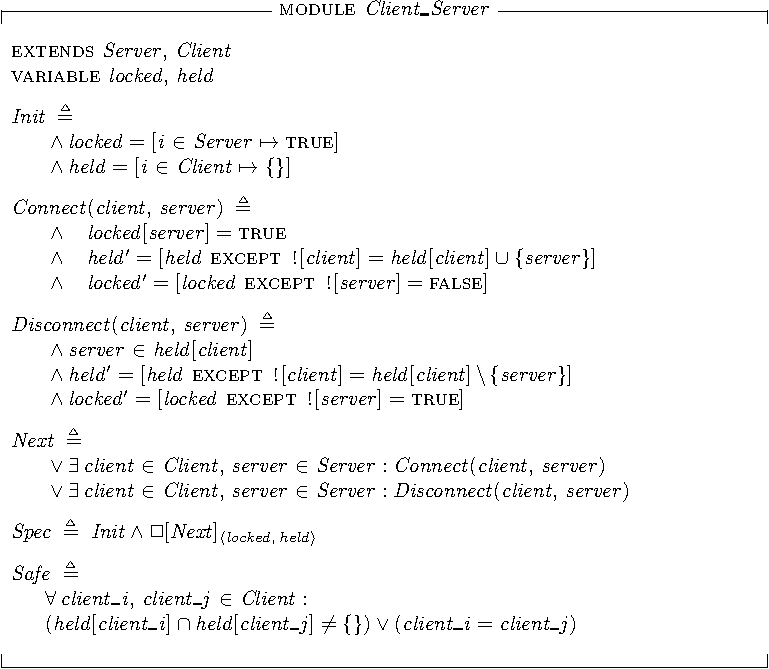
\includegraphics[width=0.8\textwidth]{figures/Client_Server.pdf}
    \caption{Client\_Server 规约}
    \label{fig:client_server}
\end{figure}

\section{\texorpdfstring{TLA\textsuperscript{+}与TLC}{TLA+与TLC}}
\subsection{\texorpdfstring{TLA\textsuperscript{+}形式规约语言}{TLA+形式规约语言}}
\href{https://lamport.azurewebsites.net/tla/tla.html}{\TLA} \cite{TLA+}是由计算机科学家 Leslie Lamport 主导开发的,基于时许逻辑TLA(temporal logic of actions)\cite{temporal}的,
在对计算机程序和系统建模,尤其是对并行系统和分布式系统建模具有广泛应用\cite{PaxosStore}的一种高级语言。
它是基于使用简单的数学语言来精确描述系统行为的理念开发的。
因此,\TLA 的表达方式和一般的编程语言有很大的不同,反而和数学语言更为接近。
\TLA 并不是一种编程语言,而是一种规约语言,它不关注协议或者系统的具体实现,从而能更高层次看到程序整体的设计。
因此,\TLA 及其工具对于消除代码中很难发现和纠错成本高昂的错误非常有用。

需要注意到的是,\TLA 是一个对程序或者系统建模的语言,为了让规约开发人员能更好地表达一个协议或系统而设计的,
并不是为了寻找归纳不变式而设计的。
尽管如此,它的语法更加丰富,以更加直观的方式表达一个协议或系统,而且在工业界应用更加广泛,使得它在寻找归纳不变式的研究中有广阔的应用。

开发者使用 \TLA 或者其他工具来对分布式协议进行建模的代码,我们将其称之为规约(specification,简称spec)。
图 \ref{fig:client_server} 展示了一个简单的 \TLA 规约,其中包含了一个简单的客户端和服务器的通信协议。
其中两个重要的谓词是 $Init$ 和 $Next$。
$Init$ 表示系统的初始状态,描述系统最开始时的状态;
而$Next$ 则是表示系统的状态是如何转移,也就是系统的状态在每个时间片后会发生怎样的变化。
谓词$Safe$ 是安全属性(safety property),一个正确定义的分布式协议规约,应当在每个可达的状态下都满足安全属性。
这个变量在自动化生成归纳不变式的研究中非常关键。
在这个规约中,还有$Connect, Disconnect$ 等这样的动作定义,使用这些定义,就像在一般的编程语言中使用函数一样,方便阅读和重复使用。
除此以外,一些规约中还有谓词 $TypeOK$,用于约束变量的类型。
另一种在自动归纳不变式生成研究中常常使用的工具,IVy,也有相似的语法和结构。
可以看到的是,\TLA 更关注系统的状态和系统状态是发生怎样的转移,对于系统状态转移的具体实现,\TLA 并不关心。
这样的描述方式和状态机非常相似。

TLC 是 \TLA 集成的模型检测工具。
除了 TLC 以外,\TLA toolbox\cite{tla+toolbox} 还集成有PlusCal\cite{PlusCal}和TLAPS用于命题证明工具,sany用于语法检查工具,
tex 用于将\TLA 美化打印的工具等,这些工具与本文所讨论的问题相关性不高,不展开讨论。

本文所述工具只接受\TLA 的规约。

\subsection{TLC模型检查器}\label{sec:tlc-apalache}
TLC既是对\TLA 规约的模型检查工具,也是一个面向规约的模拟器。
它是一个显式状态模型检查器,依照用户给出的规约和设置,搜索所有满足约束的状态和状态转移,
并在这个过程中检查安全属性和其他用户定义的谓词逻辑时时是否成立。
如果遇到错误,TLC会将错误的状态和状态转移过程输出,以便用户进行分析。

TLC可以通过使用超过32个计算机线程以获得近乎线性的加速。
它可以通过在分布式部署的计算机网络上运行来进一步加速模型检查,并提供在云系统上的轻松部署。

Apalache\cite{apalache1, apalache2}是另一由社区开发的模型检测器, 和 TLC 不同的是,Apalache 并不是通过遍历所有可能的状态来检验安全属性是否成立,而是通过 SMT solver 来检验。
它是将\TLA 规约转换为 SMT 问题,然后使用 SMT solver (如Z3\cite{z3})求解来检验安全属性是否成立。
Apalaches 是一种符号检查器,它和 SMT solver 一样基于逻辑推理和公式求解实现的。
Apalache 对\TLA 源文件的语法中引入了一些限制,
尽管没有完全支持\TLA 的所有语法,但是这方便使用 SMT 求解器进行求解。

\TLA 是一个“弱类型”的编程语言,它对变量没有严格的类型注明。
但是,Apalache 需要了解\TLA 规约中变量的类型才能工作。
尽管 Apalache 有一套自己的类型推断系统,但是,它并不能完全解决所有的类型推断问题。
这使得用户,对于某些协议,需要以注释的形式来提供变量的类型,才能交给Apalache进行处理。

\section{归纳不变式与归纳反例}
验证分布式协议的正确性,就是验证协议定义的安全属性(safety property)是否在每个可达的状态下都成立。
在 \textit{Client\_Server} 规约中,我们可以看到 $Safe$ 是一个安全属性,
它表达的是,在任何状态下,如果两个客户端同时连接有同一个服务器,那么这两个客户端是同一个客户端。
换言之,两个不同的客户端不能连接到同一个服务器。

对于简单的系统,即变量和状态不多的系统,我们可以通过遍历每一个可能的状态来验证。
但是对于稍微复杂一些的系统,尤其是越来越多的分布式系统,规模越来越大,状态也越来越复杂。
通过简单的遍历的方式来验证系统的正确性,是不现实的。
寻找一个能够蕴含安全属性的不变式,并且能够在所有可能的状态转移后保持其自身的正确性,这个不变式被称为归纳不变式。
以数学的语言表示为:
\begin{align}
    &Init \vDash Ind \label{con:init}\\
    &Ind \land Next \vDash Ind' \label{con:inductive}\\
    &Ind \vDash Safe \label{con:safety}
\end{align}
其中$Init$ 表示初始状态,$Next$ 表示状态转移,$Safe$ 是安全属性,$Ind$ 表达的是归纳不变式,
而$Ind'$表达谓词$Ind$经过状态转移后的变量的状态。
定理\ref{con:init}表明归纳不变式在初始状态下成立;
定理\ref{con:inductive}表明归纳不变式在状态转移后依然成立,具有归纳性质。
比如说,如果$Ind$在状态$s$下成立,那么在$s$的后继状态下,$Ind$依然成立;
定理\ref{con:safety}表明归纳不变式蕴含安全属性,因此,如果某个运行时可达状态满足$Ind$, 那么也必然满足$Safe$。
这是我们寻找一个这样的归纳不变式的目的,通过归纳不变式的正确性验证安全属性的正确性。
这是归纳不变式所必须满足的三个条件。

对于\textit{Client\_Server} 规约,表达式\ref{con:candidate_ind}是一个可能的归纳不变式。
\begin{align}
    &\left.A_{1} \triangleq \forall s \in  { Server }: \forall c \in  { Client }:  { locked }[s] \Rightarrow(s \notin { held }[c])\right) \\
    &{ Ind } \triangleq  { Safe } \wedge A_{1} \label{con:candidate_ind}
\end{align}

总结归纳不变式的特征,$Ind$是由$Safe$和$A_{1}$两个谓词逻辑表达式合取组成而来。
事实上,大部分规约的归纳不变式都可以表达为$Ind \triangleq Safe \wedge A_1 \wedge A_2 \wedge... \wedge A_n$的形式。
其中合取子式$A_k$是约束状态的谓词,我们将之称为引理不变式(Lemma Invariant)。
因为归纳不变式$Ind$是由这些引理不变式$A_k$组合而成的,也就是说,归纳不变式强于每一个引理不变式。
因此,引理不变式需要满足不变性,也就是在系统运行的每个状态下都成立,才能成为一个合适的引理不变式。
但是,引理不变式本身不需要满足归纳性,只需要它们和安全属性的合取结果能够满足归纳性。

对于一个谓词表达式$P$,如果一个状态$s$满足$s \models P$,但是$s$的后继状态$s_{n} \models \neg P$,
那便可以称$s$ 为 $P$的归纳反例(counterexample),揭示了$P$不是归纳不变式。
一个归纳反例往往包括两个状态,前一个状态满足谓词$P$,而后一个状态不满足谓词$P$。

\begin{figure}
    \centering
    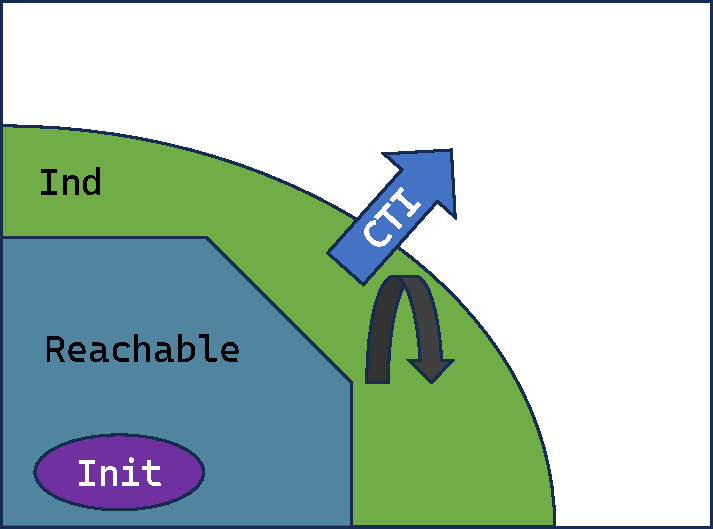
\includegraphics[width=0.4\textwidth]{figures/ind_cti.pdf}
    \caption{归纳不变式和归纳反例}
    \label{fig:ind-cti}
\end{figure}
图\ref{fig:ind-cti}形象地介绍了归纳反例以及归纳不变式、运行时可达空间和初始化空间之间的关系。
寻找归纳不变式的过程,也可以理解为通过添加新的引理不变式作为约束修剪空间,来排除归纳反例的过程。
但是,尤其是对于越复杂的系统而言,寻找归纳不变式并不是一个简单的任务。
实现归纳不变式的自动生成是形式化验证领域一个重要的研究目标,这也是本文研究的内容。

% 补充关于 返回结果和CTI的内容?

\section{强化学习}
强化学习(Reinforcement learning, RL)\cite{rl}是机器学习的一个领域,强调如何基于外部环境做出决策,以获得最大化的预期累积奖励。
是区别于监督学习和非监督学习的另外一种基本的机器学习方法。
强化学习的关注点在于寻找对未知领域的探索和对已有知识的利用之间的平衡。
它的目标是通过奖惩来控制智能体完成任务,以获得最大化的预期累积奖励,但程序无需明确告诉智能体如何完成任务。

在机器学习问题中,环境通常被抽象为马尔可夫决策过程(Markov decision processes,MDP)\cite{markov},
因为很多强化学习算法在这种假设下才能使用动态规划的方法。
但是,强化学习相较于动态规划,并不一定需要了解MDP的具体信息和全局信息,只需要通过与环境的交互,不断试错来学习。

\begin{figure}[h]
    \centering
    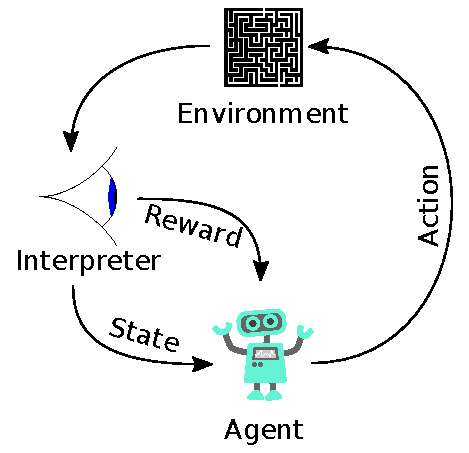
\includegraphics[width=0.4\textwidth]{figures/Reinforcement_learning_diagram.pdf}
    \caption{典型强化学习框架}
    \label{fig:rl}
\end{figure}
图 \ref{fig:rl} 展示了强化学习的框架。
在强化学习中,核心在于智能体(agent)与环境(environment)之间的交互。
环境是智能体所在的背景,它会根据智能体的动作给予奖励或惩罚,并做出状态的转移。
智能体能够感知环境的状态(State),并根据反馈的奖励(Reward)或惩罚(Reward为负值),来调整自身策略(Policy),
学习选择适当的动作(Action),以最大化长期总收益。
通过不断与环境互动,智能体根据环境的反馈不断调整策略,以期获得最大化的预期累积奖励。
实现强化学习的策略算法有很多,其中最著名的有 Deep Q Network(DQN)\cite{dqn},DDPG\cite{ddpg}等。

在本文的项目中,我们使用强化学习的方法来加速归纳不变式的生成。
我们使智能体理解\TLA 原文件的内容,让智能体合理选择生成归纳不变式的种子(seed),
并将每一次智能体选择的种子所生成的不变式的检验结果反馈给智能体,包括反例的数量,内容和生成时间等。
智能体根据这些反馈信息,调整自己的策略,以便更快地找到一个满足安全属性的归纳不变式。



\chapter{归纳不变式自动生成工具的设计}

总体上,我们的归纳不变式生成工具包括一下几个步骤:
\begin{itemize}
    \item 解析用户输入,生成用于检测三个属性的配置文件(.cfg)。
    \item 检验模块对生成模块所生成的候选不变式检验其正确性、独立性和与已有不变式析取结果的递归性,
    并解析模型检测器返回的结果,回传给生成模块;同时检验模块还需存储合适的不变式,并在得到归纳不变式时,输出结果。
    \item 基于用户输入和检验模块的结果,生成合适的不变式。
\end{itemize}

rlTLA的工作流如图\ref{fig:rltla}所示,主要分为候选不变式生成模块(Invariant Generator),候选不变式检验模块(TLC/Apalache)两个部分。
其中候选不变式生成模块接入了强化学习,训练强化模型智能体,以提高候选不变式的生成效率和准确率。
候选不变式检验模块则接入了TLC和Apalache,对生成的候选不变式进行验证,检验其正确性,独立性和与已有不变式析取结果的递归性,并将结果返回给生成模块。
在初始化阶段,候选不变式检验模块还需要生成用于检测这三种属性的配置文件(.cfg)。
目前系统接受 endive 提供的数据源,使用 endive 中的对规约人工标记的谓词,作为候选不变式的种子(seed)。
系统的输出是对一系列候选不变式的析取范式,对于系统而言,是一个包含 $Safety$ 属性的归纳不变式。

基本的逻辑结构如伪代码\ref{alg:rltla-workflow}展示。
初始化时候,候选的归纳不变式首先析取$Safety$属性,然后生成候选不变式的CTI(Counterexample to Induction)。
在每一轮的迭代中,强化学习系统都会不断地生成一个个候选不变子式,直到生成的子式在系统运行环境中是不变式,且不会被已有的不变式所包含。
这样的不变式便会加入到候选的归纳不变式中做析取,直到对候选归纳不变式生成的CTI为空,即不再有反例产生。
这说明现在系统中所有不变式的析取结果是一个包含$Safety$属性归纳不变式,系统选择将这个结果输出给用户。


\begin{figure}
    \centering
    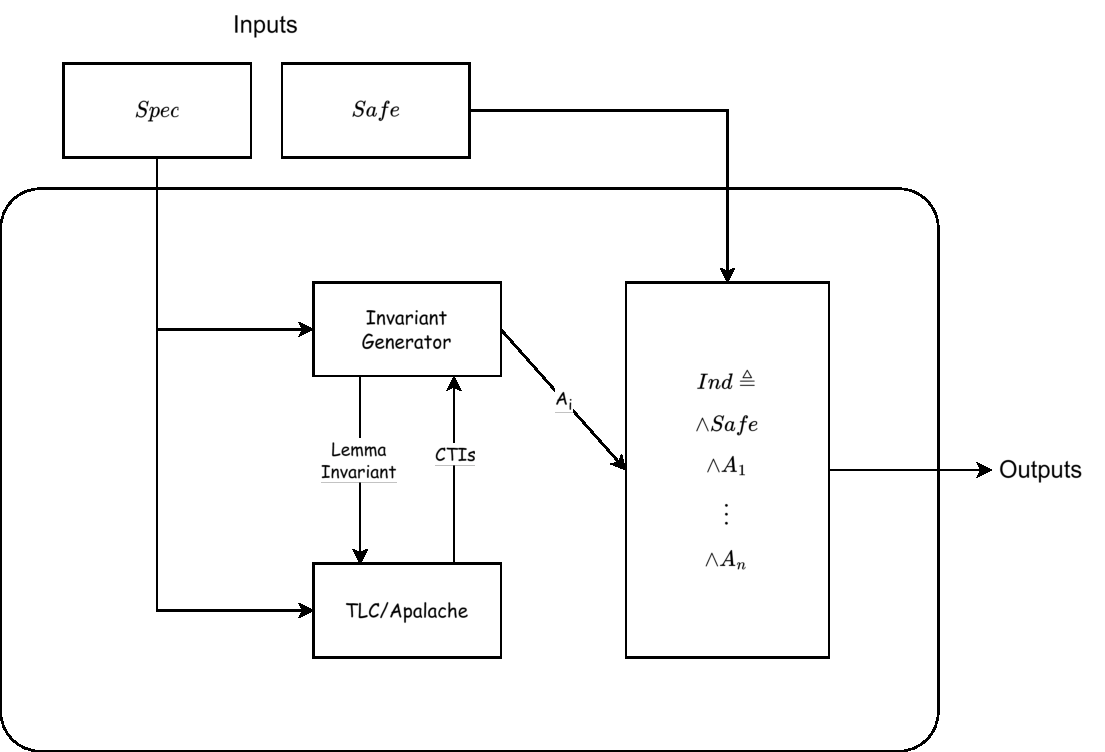
\includegraphics[width=0.7\textwidth]{figures/workflow.pdf}
    \caption{rlTLA-workflow}
    \label{fig:rltla}
\end{figure}

\begin{algorithm}
    \caption[short]{workflow of rlTLA}
    \label{alg:rltla-workflow}
    
    \begin{algorithmic}[1]
        \REQUIRE \ \\
        $M$: Finite instance of parameterized system\\
        $Safe$: Safety property
		\ENSURE \ \\
        $Ind$: Inductive invariant
		\STATE $Ind \gets Safe$
        \STATE $IndCTIs \gets GenrateIndCTIs(M, Ind)$
        \WHILE{$IndCTIs$ is not empty}
            \STATE $InvCTIs \gets IndCTIs$
            \WHILE{True}
                \STATE $Inv \gets GenerateCandidateInvariant(M, IndCTIs)$
                \STATE $InvCTIs \gets GenrateInvCTIs(M, Inv)$
                \IF{$InvCTIs$ is not empty}
                    \STATE $Continue$
                \ENDIF
                \IF {not $CheckDerivation(Ind, Inv)$} 
                    \STATE $Ind = Ind \wedge Inv$
                    \STATE $Break$
                \ENDIF
            \ENDWHILE
            \STATE $IndCTIs \gets GenrateIndCTIs(M, Ind)$
        \ENDWHILE
        \RETURN $Ind$
    \end{algorithmic}
\end{algorithm}

\section{候选不变式生成模块}

对于一个给定的规约的有限大小的实例,候选不变式生成模块的工具就是生成一系列在规约的每个状态下都成立的候选不变式,这些不变式以一阶逻辑谓词的形式存在。
为了找到这些不变式,我们使用一种基于语法合成指导的归纳不变式生成技术。
我们从输入的种子(seed)谓词中,按照强化学习模块的意愿选择一部分种子谓词,并按照语法组合成一个可能的不变式。
每个种子谓词都是针对系统状态变量的原子布尔谓词。
当然,我们也有可能采取给出种子谓词的否定,根据\TLA 的语法,我们只需要在给出的谓词前面加上否定符号 \textbf{“\~{}”}即可。
这部分的决定权交给强化学习模块,强化学习模块会根据当前的状态,选择一个合适的种子谓词,或者它的否定。

一个不变式的语法大致可以表达为:
\begin{align}
    <lemma> &: = <quant>:<expr>   \\
    <quant> &:= \forall x\ \backslash in\ SetA | \exists y\ \backslash in\ SetB \\
    <expr>  &:= <seed>| \sim<seed> | <seed> \wedge <seed>
\end{align}
注意到本文中所提及的大部分的\TLA 规约都带有存在量词和全程量词,我们直接将这一部分量词当作输入的一部分。
尽管可以带来多余的量词表达式,但是这部分量词并不会对整个谓词的布尔值带来实际的影响,这部分多余的量词可以不做处理。
另外,我们对于候选不变式内部每个小的谓词之间的连接方式统一选择了合取符号“$\vee$”。
这是因为,一方面在逻辑表达上已经足够完备\cite{or-complete},另一方面,这也可以帮助了我们简化问题,缩小了搜索不变式的空间。


\section{强化学习在生成模块中的应用}

本文的目的是希望研究强化学习在自动的归纳不变式生成过程中的应用。
强化学习是一种通过智能体和环境的交互,智能体通过观察环境的状态,采取行动,获得奖励,来学习如何在环境中获取最大的奖励。
在本文中,强化学习被应用于生成归纳不变式的各个析取子式,也就是候选不变式。

强化学习模块接受\TLA 协议和检验模块对于本身生成的候选不变式的检验结果,修改策略,生成更加合理的候选不变式。
强化学习模块的输入是一个状态,输出是一个动作,动作是对于种子谓词的选择与否,和是否选择它的否定。

强化学习模块的目标是生成一个合适的候选不变式,这个候选不变式在规约的每个状态下都成立,且不会被已有的不变式的析取结果包含。
这个过程是自动化的,但人可以通过挑战对强化学习智能体在每个状态下的每个动作的选择给出合适的奖励或者惩罚,以指导智能体学习到
一个合适的策略,并应用到后续的候选不变式生成中。

最高的奖励应当给予给出最终的归纳不变式的行为,也就是给出了一个不变式,使得它和前面所有不变式的析取结果是归纳不变式的行为。
当强化学习模块给出一个不变式的时候,也应当给出一定的奖励。给出一个不变式,尤其是给出第一个不变式,往往是一个十分困难的过程。
而且,这一步也是实现最终目标的关键。因此,我们应当给予一定的奖励,以鼓励智能体继续学习。

生成一个已经被已有不变式包含的不变式,尽管没有意义,但也体现出智能体如何寻找不变式的能力,因此也应当给予一定的奖励。
这个奖励的值很小,但是也是必要的。因为这个过程是一个逐步的过程,智能体需要不断地尝试,才能找到一个合适的不变式。
但是,为了防止智能体的惰性,我们不允许智能体在已有的不变式上简单的合取上一个谓词,然后给出这个谓词作为候选不变式,
同样的,不允许在一个错误的不变式上去除掉一些谓词,以得到候选不变式。
这是简单的重复,是没有意义的,我们对智能体的这种行为应当给予惩罚。


\section{候选不变式检验模块}

候选不变式检验模块需要调用模型检查器,并且需要将输出解析,并将结果返回给生成模块。
对于候选不变式的检验,可以分为三个部分,分别是正确性、独立性和多个不变式析取结果的递归性。
引理\ref{con:inv_correct}表达了候选不变式的正确性,即候选不变式在规约的每个状态下都成立。
引理\ref{con:inv_indepence}表达了候选不变式的独立性,即新生成的候选不变式不能被已有的不变式的析取结果包含。
\begin{align}
    &Spec \triangleq Init \wedge [Next] \\
    &Spec \vDash Inv \label{con:inv_correct} \\
    &Spec \wedge IndCand \nvDash Inv \label{con:inv_indepence}
\end{align}

检验候选不变式的正确性,就是检验每个候选不变式是否在规约的每个状态下,布尔值都为真。
这个问题虽然简单,但是直觉上可能需要遍历许多状态和多个状态转移轨迹,可能需要很长的时间。
但是实际上,很多的不正确的候选不变式在规约的某个比较容易到达的状态被验证器检验出来,便可以退出了。
一个正确的不变式,尽管现在还不能成为归纳不变式,但是它确实我们需要归纳不变式的开始。

检验不变式的独立性时,我们需要验证新生成的候选不变式是否能被已有的不变式的析取结果包含。
检验不变式的独立性十分重要,尤其是对于指导强化学习生成候选不变式,
因为如果新生成的候选不变式能被已有的不变式的析取结果包含,那么生成模块为了得到更高的奖励,
会多生成这样的候选不变式,这样会导致不变式的重复,析取的结果的约束能力也不能加强,对状态空间不能做出有价值的修剪,
这样的不变式便是没有意义的。系统也就无法找到一个合适的归纳不变式。

检验归纳不变式的递归性,是我们工作的终点。
如果多个不变式的析取结果具有递归性,那么我们可以将这个析取结果作为归纳不变式,我们可以将这个结果输出,并结束这个循环。
对于不变式的递归性质,在引理\ref{con:init}和\ref{con:inductive}中已经提及。
归纳不变式需要包含所有的初始状态,并且,从归纳不变式约束的状态出发,进行状态转移,新生成的状态也需要满足归纳不变式。
另外,我们最根本的目的是证明安全属性,那么,归纳不变式需要蕴含安全属性。



\chapter{归纳不变式自动生成工具的实现}

本章节基于设计方案,详细介绍了归纳不变式自动生成工具的实现细节,包括块之间的交互,以及模块的具体实现。

\section{候选不变式检验模块}

候选不变式检验模块主要负责对生成的候选不变式进行验证,检验其正确性,独立性和与已有不变式析取结果的递归性。

候选不变式检验模块接入了TLC和Apalache,用户可以选择其一对生成的候选不变式进行验证。
TLC 和 Apalache 是两个常见的面向\TLA 规约的模型检查工具(model checker),可以使用相似的配置文件对规约进行验证,
但是,两者的结果输出格式不同,需要做分别处理。

此外,由于Apalache需要用户对协议中的变量和常量做出类型的注释,因此,目前能够提供的测试集中大多数的规约都无法使用Apalache进行验证。
在系统实现时,我们默认状态下使用TLC作为系统的模型检查器。
当然,在条件允许时,用户可以设置系统的参数来使用Apalache作为系统的模型检查器。

\subsection{model checker的配置文件和运行选项}

对于图\ref{fig:client_server}中的规约,TLC 和 Apalache 会使用默认的配置文件进行验证,
即以 $INIT$为初始状态,$NEXT$ 为状态转移关系,在状态变化的过程中验证 $Safe$ 安全属性的正确性。
用户也可以指定使用其他配置文件,以验证从不同状态出发和不同状态转移条件下的用户定义的不变式的成立与否。
比如说需要验证的不变式,可以放在$INVARIANT$ 字段下。
我们可以简单的理解为,TLC可以判断$INIT \wedge NEXT \vDash INVARIANT$ 是否成立。
对于一些常量,用户也可以通过配置文件进行定义,以便模型检查器能够正确地理解规约的含义。

我们希望TLC和Apalache为我们验证生成模块生成的候选不变式的正确性,独立性和与已有不变式析取结果的递归性。
在验证过程中,我们希望模型检查器能够输出验证结果,以及验证过程中的反例(Counterexample)。

在验证这三个性质的过程中,统一的是我们不需要更改$NEXT$的取值,将一直选择规约中的参数$Next$。
同样不变的还有对常量$CONSTANTS$的定义和初始化,它们在规约每个状态下都保持着一开始定义时的值。
我们直接选择已有的定义,这一般设计用户如何使用这些规约,这些参数在验证时不需要也不方便更改。

在检验生成的候选不变式正确性时,我们需要将$INVARIANT$替换为我们生成的候选不变式,$INIT$选择规约中的$Init$。
我们以着这样的配置文件验证在规约运行的每个状态下,候选不变式是否成立。
只有一个在规约约束的系统运行的每个状态下,候选不变式都成立,我们才有可能将这个候选不变式变成归纳不变式的一部分。

验证候选不变式的独立性,就是验证已有的不变式的析取结果是否可以包含新生成的候选不变式。
我们已经知道,规约运行的每个状态下,$IndCand$的每个析取子式都是正确的,也就是说,规约所约束的状态是现有的不变式所约束的状态的子集。
为了加速验证新生成的候选不变式的独立性,我们只需要从$IndCand$约束的状态出发,也就是将配置文件中的$INIT$选择为 $IndCand$ 进行采取原始的状态转移。
正如引理\ref{con:inv_indepence}所表达的,
如果产生的所有新状态下,新生成的候选不变式都成立,那么可以说明新生成的候选不变式不能对状态空间产生新的约束,即新生成的候选不变式不是独立的。
这样的不变式是不应该被添加到归纳不变式中的。

验证$IndCand$的递归性,就是验证从$IndCand$出发的每个状态,都重新回到$IndCand$中,也就是验证$IndCand$的正确性。
所以,我们将$INIT$和$INVARIANT$设置为$IndCand$。
验证这一性质,一般发生在我们已经验证了一个不变式的正确性和独立性后,且需要把这一不变式析取进$IndCand$中。

我们需要将新生成的不变式放到一个新的文件中,并使用关键字\textbf{EXTENDS} 将原有规约中的定义引入。
这样,我们就可以在新的文件中使用原有规约中的定义,和引入生成模块生成的候选不变式。
由于新的\TLA 文件中有着相似的结构,在验证同一个性质时,配置文件是可以复用的。
所以我们在系统运行之初就定义好配置文件中的内容,并写入硬盘供TLC/Apalache使用。

在使用TLC验证时,我们还需要关注诸多选项。
\textbf{"-config"}是我多样化使用TLC和apalache的关键,通过这个选项,我们可以指定TLC和Apalache的配置文件,以检验不变式的不同性质。
\textbf{"-deadlock"}选项用于检查是否存在死锁状态,如果选择了这个选项,那么TLC就不会检验死锁。
由于我们的目的是检验不变式的一些性质,所以我们不需要检验死锁,并选择了这一选项。
\textbf{"-depth"}选项揭示了TLC的状态空间搜索的深度,我们可以通过这个选项来控制TLC的搜索深度,在不同情况下,我们会选择不同的深度。
例如在检验递归性时,只需要将深度设置为2,即经过一步转化后$IndCand$ 是否还满足。

\subsection{model checker 的调用和结果解析}
本项目的代码主要基于Python实现,然而不论是TLC还是Apalache,都是Java实现的模型检查器,且没有可以直接调用的Python接口。
因此,我们需要通过Python的subprocess库来调用Java程序,并通过解析Java程序的命令行输出结果来获取验证结果。
在验证不同性质的时候指定好不同的配置文件并调整好不用的运行参数。

对于结果的解析,主要是将TLC或Apalache的输出结果进行解析,去除无用的信息,将有用的信息交给强化学习模块,以便强化学习模块调整策略,提高生成的候选不变式的正确性。
TLC和Apalache尽管两者有着不同的输出格式,但是他们的功能其实是一致的,都是将出现不变式错误时的状态,以及前序状态,也就是错误轨迹(error trace)。
错误轨迹的每一个节点都是一个状态,表达的是在这个状态下,各个变量的值。
TLC会以析取范式的形式将各个变量的值表达出来,而Apalache默认使用的json文件格式,将各个变量的值以键值对的形式表达出来。
我们需要将这些信息解析出来,以便强化学习模块能够理解这些信息,调整生成的候选不变式。


\section{候选不变式生成模块}

生成模块是本项目的关键,它负责生成候选不变式,检验模块是为生成模块服务的。
不同于以往的归纳不变式生成工具,使用随机枚举的方式生成候选不变式,我们引入强化学习来提高我们枚举的效率和成功率。




\chapter{运行试验和结果分析}\label{chap:run-analysis}

\section{运行结果}

以{Client\_Server}规约为例, 一个典型的配置文件如下:
\begin{lstlisting}[label={lst:config},caption={配置文件}]
{
    "preds"  :  [
        "<<VARR,VARP>> \\in match",
        "<<VARI,VARR>> \\in request_sent",
        "<<VARJ,VARR>> \\in request_sent",
        "<<VARI,VARP>> \\in response_sent",
        "<<VARJ,VARP>> \\in response_sent",
        "<<VARI,VARP>> \\in response_received",
        "<<VARJ,VARP>> \\in response_received",
        "VARI=VARJ /\\ match = match",
        "ResponseMatched(VARI,VARP)"
    ],
    "preds_alt" : [],
    "safety"  :  "Safety",
    "constants"  :  "CONSTANT\nNode = {n1,n2,n3}\nRequest = {r1,r2}\nResponse={p1,p2}\nn1 = n1\nn2 = n2\nn3 = n3\nr1 = r1\nr2 = r2\np1 = p1\np2 = p2\n",
    "constraint"  :  "",
    "quant_inv"  :  "\\A VARI \\in Node : \\A VARJ \\in Node : \\A VARR \\in Request : \\A VARP \\in Response : ",
    "quant_inv_alt"  :  null,
    "quant_vars": [],
    "model_consts"  :  "CONSTANT n1,n2,n3,r1,r2,p1,p2",
    "symmetry" : true,
    "typeok"  :  "TypeOK",
    "simulate"  :  true      
}
\end{lstlisting}

\rltla 和endive 使用相同的配置文件。

本文得到的运行数据,包括对endive的运行数据的机器配置如下:
\begin{itemize}
    \item CPU: AMD Ryzen 9 5950X 16-Core Processor @4.6GHz
    \item 内存: 128GB
    \item 操作系统: Ubuntu 22.04
    \item 显卡: Tesla V100-SXM3-32GB
    \item TLC版本: 2.15
\end{itemize}
运行结果数据如表\ref{tab:result}展示,其中数据取三次运行时长中位数的结果,内存数据采用Memray工具的最大内存占用值。

\begin{table}[!htbp]
    \centering
    \renewcommand{\arraystretch}{1.3} % Increase the row height
    \caption{\rltla 和endive 运行结果对比}
    \begin{tabular}{p{0.17\textwidth}p{0.1\textwidth}p{0.1\textwidth}p{0.1\textwidth}p{0.1\textwidth}p{0.1\textwidth}p{0.1\textwidth}}

        \toprule
        \multirow{2}{*}{\textbf{规约名称}} & \multicolumn{3}{c}{\textbf{\rltla }} & \multicolumn{3}{c}{\textbf{endive}}   \\ \cline{2-7}
          & \textbf{耗时/sec}   & \textbf{内存占用/GB}  & \textbf{lemma 数量}   & \textbf{耗时/sec} & \textbf{内存占用/MB} & \textbf{lemma数量} \\ 
        \midrule
        TwoPhase   & 25.49    & 13.54   & 13  & 30.02    & 120.04   & 9      \\
        client\_server\_ae & 100.38 &12.61 &2 & 45.13 & 85.49 & 1 \\
        simpele\_election & 65.68 & 12.39 & 6 & 19.26 & 61 & 3 \\
        learning\_switch\_i4	& 93.34	& 12.12	& 1	& 147.07 & 124 & 1 \\
        consensus\_epr &	900.22 & 14.46 & 7 & 513.83	& 196 & 7 \\
        sharded\_kv	& 164.73 & 15.03 & 9 & 181.04 & 222.4 & 5 \\
        \bottomrule    
    \end{tabular}
    \label{tab:result}
\end{table}

\section{结果分析}
对比endive的运行结果,在大多数规约上\rltla 不具有优势。
\rltla 的主要内存占用为强化学习模型和网络模型的内存占用,endive没有相关的内容。
相较而言,我们的工具生成归纳不变式寻找的引理不变式更多,效率较低。
对于这一现象的现象的解释,我认为是强化学习智能体在一开始尝试时会更偏向于选择已有的不变式比较相似的不变式,
但是在系统的提示下,相似的不变式往往不能得到很好的奖励值,于是系统便会在更加稀疏的区域寻找不变式。
并且没有考虑每个不变式所能消除的归纳反例的数量,只要某个不变式能消除归纳反例,就会被加入。
而endive则是通过基于候选不变式能杀死归纳反例的个数进行选择,事实上,它可能验证的不变式的个数更多。
这样的结果导致了,我们的工具会生成更多的相近不变式,但是,这不妨碍我们的工具生成最终正确的归纳不变式。

另外,系统运行的总体时间相较于endive偏长。
一方面,\rltla 所需的轮次比endive 更多。TLC/Apalache 还没有面向python 的接口,这导致我们需要通过调用命令行的方式来调用TLC/Apalache。
一次调用和数据解析的时间随状态的多少和需要检查不变式的多少指数级增加。
另一方面,强化学习模型的训练时间和网络的向前向后传播也是一个不可忽视的因素。
但相较于随机遍历,以\textit{simple\_election}为例,拥有12个用户定义谓词,对于长度小于4的候选不变式,大概需要遍历接近万次。
然而我们的工具,遍历的次数在千次左右,在效率上有显著的提升。

\section{对强化学习的消融实验}
为了证明强化学习模块在归纳不变式生成过程中起到了作用,我们在Two Phase协议上进行了强化学习模块的消融实验,我们使用完全随机的seed选择过程代替强化学习。
图\ref{fig:all}展示我们的实验结果,其中,图\ref{fig:inv}表示截至目前为止,每轮生成的候选引理不变式通过不变式检查的频率,图\ref{fig:ind}表示最终加入到归纳不变式候选集合中的概率。
以上图表表明,强化学习模块在归纳不变式生成过程中起到了积极的作用,提高了候选引理不变式的质量。
\begin{figure}[htb]
    \centering
    \subfloat[引理不变式命中率]{
        \label{fig:inv}
        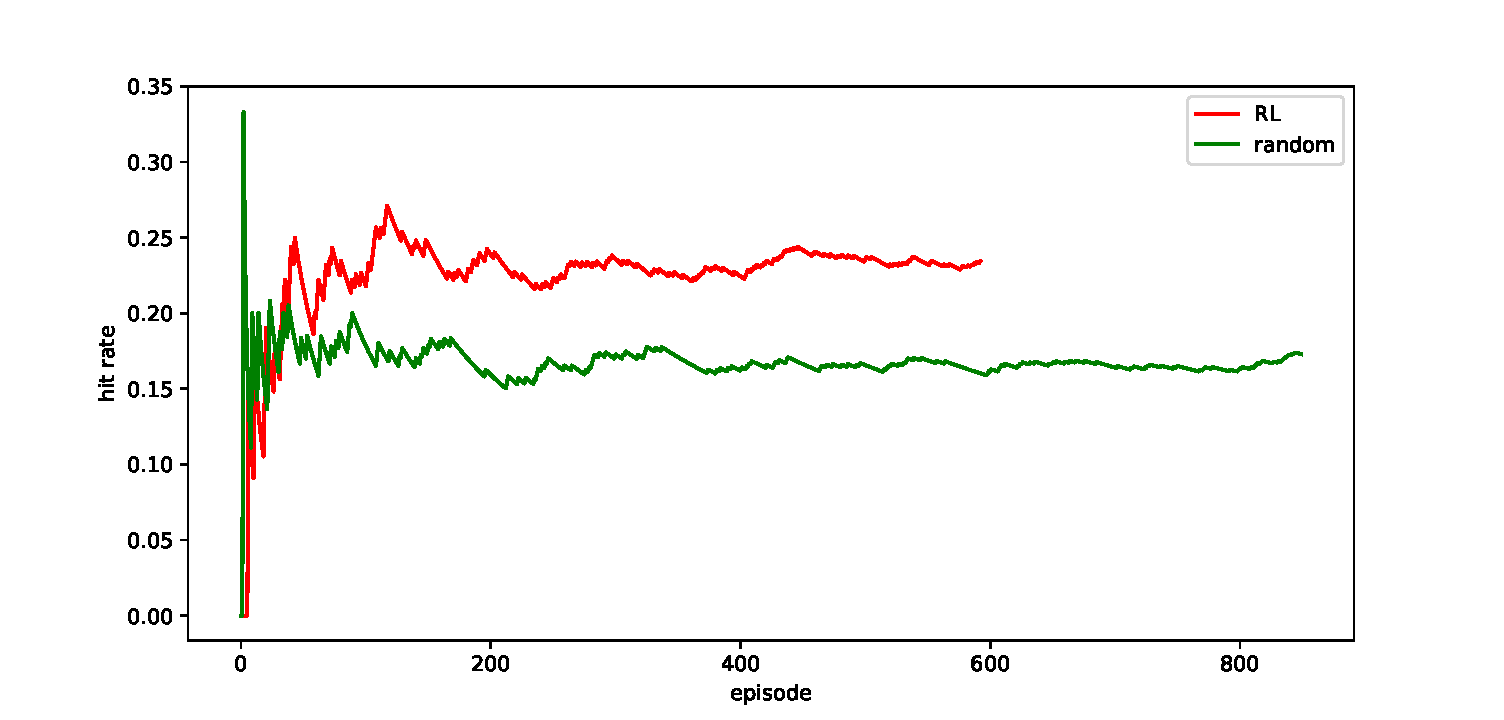
\includegraphics[width=0.8\linewidth]{figures/inv.pdf}
    }\hfill
    \subfloat[归纳不变式命中率]{
        \label{fig:ind}
        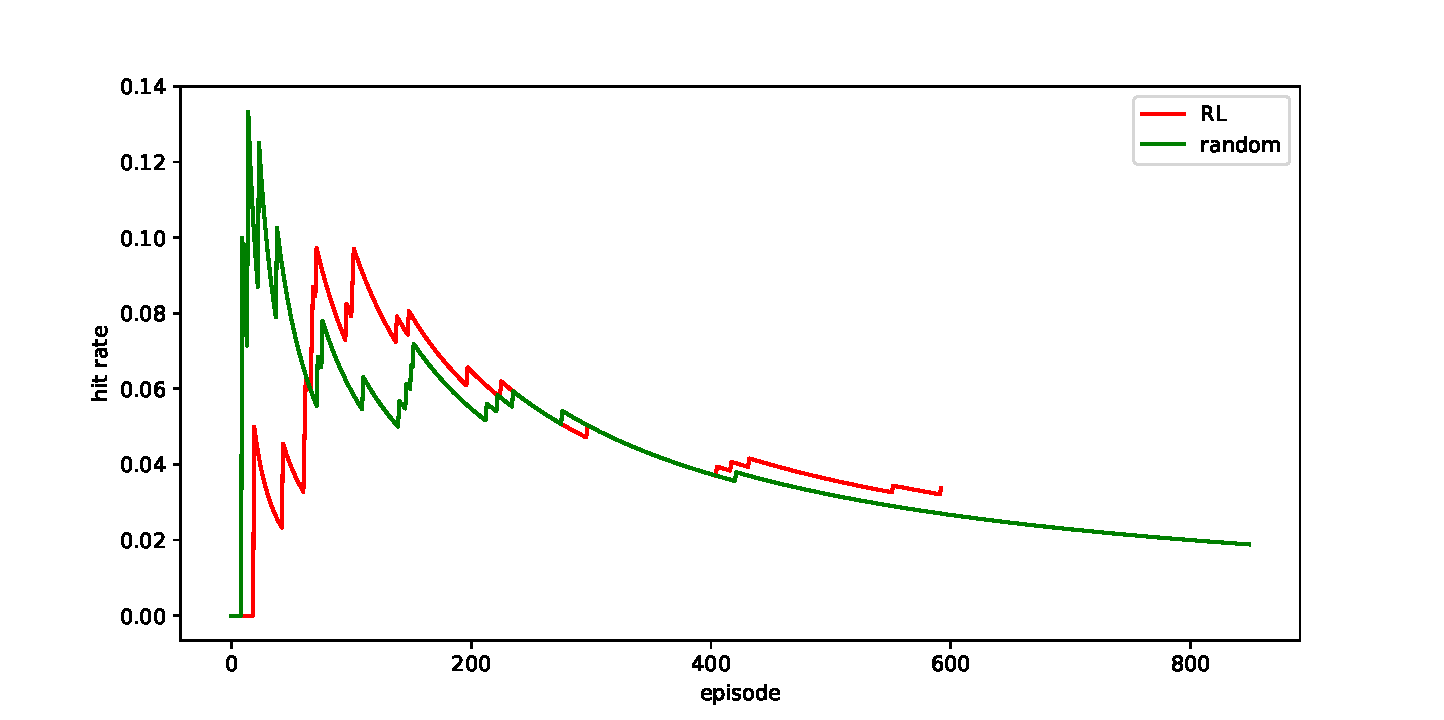
\includegraphics[width=0.8\linewidth]{figures/ind.pdf}
    }\hfill
    \caption{强化学习选择和随机选择的命中率}
    \label{fig:all}
\end{figure}


\chapter{总结与分析}\label{chap:conclusion}
本章对论文工作进行了总结,并展望了未来可能的优化和改进方向。
\section{工作总结}
本文主要目的是验证机器学习,尤其是强化学习在对分布式系统规约的归纳不变式生成领域中的可行性和有效性。

本文在\TLA 的语言平台上,实现了一个基于强化学习的归纳不变式生成系统。
首先,介绍了系统设计的预备知识和理论基础,然后介绍了\rltla 的系统体系结构的设计和实现,最后展示了运行数据,并对结果进行分析。

\TLA 相较于 IVy 更加复杂,其中存在灵活多样的数据结构,同时也支持任意的嵌套来表达规约。
这对开发人员在设计阶段表达系统的行为和状态转移关系提供了很大的便利,但这点对于归纳不变式生成工具的设计并不友好。

实现上,本文依靠于\TLA 源文件和 endive 对于\TLA 解析和人工识别的假设作为输入,基于 try-and-error 的生成思路,
采用强化学习的方式生成候选不变式,通过模型检查器验证候选不变式的正确性,独立性以及当前所有候选不变式合取结果的递归性,最终生成归纳不变式。
这一生成思路和大部分的归纳不变式生成工具类似,但是在实现上,本文寄希望于强化学习以提高生成效率。

本文基于LIPuS \cite{LIPuS} 对结构化程序寻找循环不变式的研究开发了一套面向\TLA 的强化学习模型。

本文使用TLC和Apalache对生成的候选不变式进行验证,检验生成的候选不变式的正确性,独立性和与已有不变式合取结果的递归性,并将结果返回给强化学习模块。
TLC和Apalache没有提供python的接口,本文通过调用命令行的方式调用TLC和Apalache,并通过对命令行结果的解析,获取验证结果。

在测试部分,本文使用 endive 提供的测试用例对系统进行测试,并和endive进行了比较,
验证了强化学习在面向分布式系统规约的归纳不变式生成工作中具有可行性和有效性。

\section{未来展望}
由于时间和能力的限制,本文所实现的系统的性能和实现方式上有许多不足,存在大量的改进空间。

目前,和endive一样,\rltla 还以来于一些人工的输入,即一些人工识别的假设(predicates)
,这些假设的得到是依赖于人脑对于 \TLA 规约理解,尤其是对每个 Action 进行调用时参数类型的理解。
如果要自动化地识别和生成这些假设,也是一个复杂的工作,目前系统还不具备这项能力。
与此同时,人脑的参与可能带来效率的下降和不可预计的错处的出现。
另一方面,如同 endive 的通过机械搜索的方式,可能获得比强化学习更快的生成效率,强化学习的优势难以发挥。
未来需要实现一个功能更加丰富的静态分析工具,以自动提取出 \TLA 规约的语义信息,包括 Action 的"函数签名"等,
以帮助强化学习模块更好地理解 \TLA 规约和生成合适的候选不变式。

近些年,大语言模型的流行,使得自动归纳不变式生成有了更多可能。通过将协议交给大语言模型进行学习,可以更好地理解协议的行为。
或者,大语言模型也许可以直接应用于归纳不变式的生成工作,这是一个值得尝试的方向。

其次,目前提供给系统可以选择的谓词对于系统来说都是平行的,并没有考虑谓词的子式以及谓词之间的关系。
系统也无法考虑给出的这些谓词表达式之间,以及每个可能的候选不变式之间的关系。
这有可能导致系统生成的候选不变式之间存在冗余,或者存在矛盾,导致系统的效率降低。
另外,目前系统设计上,一次只生成一个可能的候选不变式,
这两方面因素,导致了对于每一次的生成的候选不变式的检查,都需要调用1-3次模型检查器进行检查,这往往很花时间,导致系统的效率较低。
这也是目前在效率上较 endive 等工作有所不足的地方。

基于\TLA 的归纳不变式的生成是一个复杂的问题,在这一领域的研究不是十分充足,可以参考和对比的工作较少。
目前,对于基于\TLA 的归纳不变式生成工具还没有统一的测试集合,也没有十分充足的测试用例。
这导致我们一方面很难评估系统的效率,另一方面,也很难提供给强化学习模块足够的训练数据。
在 endive 的测试集合下,一个归纳不变式常常只需要不超过10个子式合取而来。
在这一背景下,强化学习的效率并不理想,常常带来相较于 endive 等工作提供的搜索算法更高的开支和更低的效率。



% 生成参考文献页
\printbibliography

\begin{acknowledgement}
时光荏苒,四年的时间很快过去了。2020年9月3日大清早,拖着行李走进南大校门,穿过教学楼和一组团主干道的场景还历历在目,仿佛就在昨天,如今却快要到达四年本科学习的终点,走向下一段旅程。
本科四年,求学生涯,乃至人生到此的所有阶段,都离不开许多人的帮助和支持。

感谢父母,祖父母对我的养育之恩,对我生活和求学的支持。是他们的付出,让我有成长学习的环境。

感谢魏恒峰老师在学习生活上的指导。是他带领我进入科研的大门,让我了解分布式系统验证和形式化方法。

感谢诸位朋友的陪伴,开导,帮助和建议,人生因为你们而丰富多彩。

感谢党和国家对教育事业的支持。感谢南京大学,以及诸位老师,工作人员为我们提供了一个良好的学习环境。

\end{acknowledgement}
\appendix
\chapter{endive 对 simple\_election 的验证结果}\label{app:endive_simple_election}
\begin{lstlisting}
  
Inv219_1_0_def == \A VARS \in Acceptor : \A VARPA \in Proposer : (VARPA \in start) \/ (~(<<VARS,VARPA>> \in promise))
Inv136_1_1_def == \A VARPA \in Proposer : \E VARQ \in Quorum : (ChosenAt(VARQ,VARPA)) \/ (~(VARPA \in leader))
Inv200_2_2_def == \A VARS \in Acceptor : \A VARPA \in Proposer : \A VARPB \in Proposer : ((VARPA=VARPB) /\ promise = promise) \/ (~(<<VARS,VARPA>> \in promise)) \/ (~(<<VARS,VARPB>> \in promise))

\* The inductive invariant candidate.
IndAuto ==
  /\ TypeOK
  /\ Safety
  /\ Inv219_1_0_def
  /\ Inv136_1_1_def
  /\ Inv200_2_2_def
\end{lstlisting}

\chapter{Client\_Server 规约的配置文件}\label{app:client_server_config}
\begin{lstlisting}
{
    "preds"  :  [
        "<<VARR,VARP>> \\in match",
        "<<VARI,VARR>> \\in request_sent",
        "<<VARJ,VARR>> \\in request_sent",
        "<<VARI,VARP>> \\in response_sent",
        "<<VARJ,VARP>> \\in response_sent",
        "<<VARI,VARP>> \\in response_received",
        "<<VARJ,VARP>> \\in response_received",
        "VARI=VARJ /\\ match = match",
        "ResponseMatched(VARI,VARP)"
    ],
    "preds_alt" : [],
    "safety"  :  "Safety",
    "constants"  :  "CONSTANT\nNode = {n1,n2,n3}\nRequest = {r1,r2}\nResponse={p1,p2}\nn1 = n1\nn2 = n2\nn3 = n3\nr1 = r1\nr2 = r2\np1 = p1\np2 = p2\n",
    "constraint"  :  "",
    "quant_inv"  :  "\\A VARI \\in Node : \\A VARJ \\in Node : \\A VARR \\in Request : \\A VARP \\in Response : ",
    "quant_inv_alt"  :  null,
    "quant_vars": [],
    "model_consts"  :  "CONSTANT n1,n2,n3,r1,r2,p1,p2",
    "symmetry" : true,
    "typeok"  :  "TypeOK",
    "simulate"  :  true      
}
\end{lstlisting}

\end{document}